
\subsection{Phase I: Gallium Drop Method}


\begin{wrapfigure}[12]{r}{0.5\linewidth}
	\begin{subfigure}[b]{0.5\textwidth}
		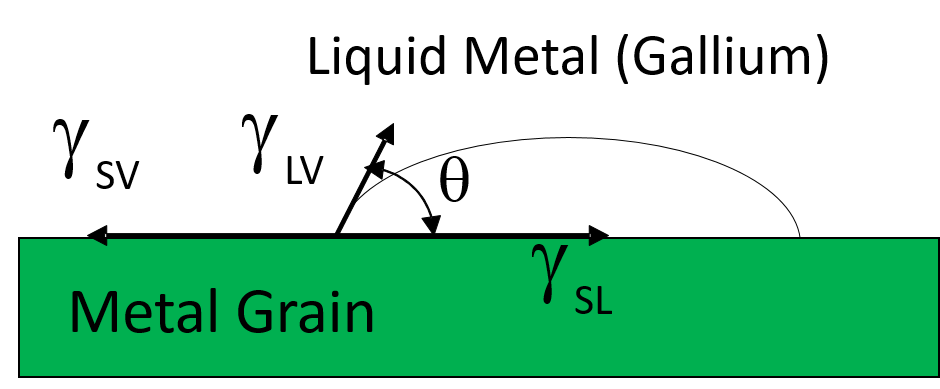
\includegraphics[width=\textwidth,trim={0 0 0 2cm}]{youngs-ga}
	%	\caption{Interfacial tensions on Ga drop on solid surface}
		\label{fig:youngs-ga}
	\end{subfigure}
	%add desired spacing between images, e. g. ~, \quad, \qquad, \hfill etc. 
	%(or a blank line to force the subfigure onto a new line)
	\begin{subfigure}[b]{0.5\textwidth}
		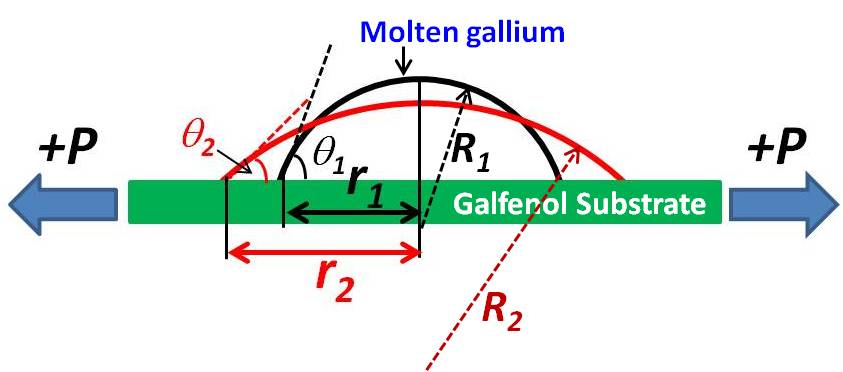
\includegraphics[width=\textwidth,trim={0 2cm 0 0}]{thermal-expand-drop}
	%	\caption{Thermal expansion of drop}
		\label{fig:thermal-expand-drop}
	\end{subfigure}
	\caption{Schematics indicating notation used and contact angles $\theta_{i}$, radii of drop-solid contact area $r_{i}$, and radii of curvature for a spherical drop $R_{i}$, for two temperatures as thermal expansion induced tension $P$ strains the substrate.}
	\label{fig:therm-exp-ga}
\end{wrapfigure}
The first technique employs measurement of contact angles and drop size of a liquid metal, gallium, resting on a metal surface as the metal is heated. Changes in surface tension will be introduced by controlled thermal expansion of the substrate at temperatures ranging from $\sim$30-100\degree C to give mobility to the molten gallium drop.
% and ensure that surface heterogeneities do not obscure the drop-substrate contact angle. 
A video system will be used to precisely quantify dimension changes in substrate and liquid metal drop during thermal expansion will be used. The surface energy of the free surface of the substrate as a function of temperature, \gamSV(T), can be related to thermal-expansion-induced changes in the liquid gallium drop contact angle $\theta$, the radius $r$ of the liquid gallium drop in contact with the metal surface, and the height $h$ of the hemisphere of liquid gallium. 

These can be modeled as a tensile load +$P(T)$ caused by substrate thermal expansion (Figure \ref{fig:therm-exp-ga}), which effectively appears as a uniform radial expansion of the planar solid surface as temperature increases. By letting the system equilibrate at different temperatures before measuring liquid drop geometry, terms due to variation in thermal energy and variation of the total Gibbs free energy vanish. Then, the interface energy between the substrate solid and the liquid gallium drop, \gamSL, is given as \gamSL$=P(T)/2\pi r$. The uniform tension introduced by thermal expansion of substrate can be expressed as:
\begin{equation}\label{uniform-tension}
	P(T) = E_{sub}\alpha_{sub}(T-T_{mp})
\end{equation}
where $T_{mp}$ is the melting temperature of gallium, $E$  is the substrate Young’s modulus, and $\alpha$ is the linear thermal expansion coefficient. A linear function can be used to write the gallium-air interfacial tension a function of temperature, \gamLV $= a-b(T-T_{mp})$, where \textit{a} and \textit{b} are positive constants found experimentally.\cite{Hardy1985,Alchagirov2005} Putting the terms for \gamSL and \gamSV into \hyperlink{youngeqn}{Young’s equation}\cite{Rudawska2009,Tadmor2004}:
\begin{equation*}%\label{youngs-eqn-ga1}
	\gamma_{SV} =  \frac{E_{sub}\alpha_{sub}(T-T_{mp})}{2\pi r} + \left[a-b(T-T_{mp})\right]\cos\theta
\end{equation*}

A relationship between the variable radius $r(T)$ associated with the area of the circular region of solid-liquid contact $A_{SL}(T)$, the contact angle $\theta(T)$ and the volume $V$ of the spherical cap formed by the drop is derived next. To determine the radius $r(T)$, the geometric relationships based on the radius of curvature $R(T)$ of a sphere is mapped onto the hemispherical liquid cap. The drop is modeled as being part of a sphere whose radius is $R(T)$. It is assumed that he volume $V$ of the drop is the volume of the spherical cap, and remains constant. The radius $R(T)$ can then be expressed in terms of the volume and the angle:
\begin{equation*}\label{drop-geom}
	R(T) = V^{1/3} \left[\frac{\pi}{3} \left(2-3\cos\theta(T)+\cos^{3}\theta(T)\right)\right]^{-1/3}
\end{equation*}
Using the relation $r(T)=R(T)\sin\theta(T)$ (i.e. $\theta=$0\degree corresponds to complete wetting of the surface and at $\theta=90$\degree,  $r=R$) the following formula for surface energy as a function of temperature $T$ and contact angle $\theta(T)$ (shown as $\theta_{T}$) is:
\begin{equation}\label{youngs-eqn-ga}
	\gamma_{SV} =  \underbracket{\frac{E_{sub}\alpha_{sub}(T-T_{mp})}{2\pi}\left[\frac{\pi\left(2-3\cos\theta_{T}+\cos^{3}\theta_{T}\right)}{3V\sin^{3}\theta_{T}} \right]^{1/3}}_{\text{\gamSL(T)}} + \underbracket{\left[a-b(T-T_{mp})\right]}_{\text{\gamLV(T)}} \cos\theta_{T}
\end{equation}
This gives the surface energy \gamSV of specific grains as a function of temperature by measuring $T$ and $\theta$ at thermal equilibrium.

One of the challenges in developing this new surface energy measurement capability is the need to expose the surface of the metal substrate shielded by surface oxides. The following strategies for removing of oxide layer and preventing of natural oxidation to increase the accuracy of measurement will be employed independently and in combination:
\begin{outline}
	\1 A flux used in high-temperature metal joining processes plays roles of dissolving of the oxides on the metal surface and preventing of re-oxidation as a chemical agent.
	\1 Colloidal silica polishing with nano-sized particles, such as is used for precise surface observations, like EBSD scans, which require clean surfaces to accurately detect patterns.
	\1 Electro-polishing is effective for passivation of clean surfaces after chemical and mechanical polishing for removal of surface oxides. 
\end{outline}
%Results using the proposed approach were to be validated through comparison of results for oriented single crystals with published theoretical values for pure metal elements of a specific crystallography (e.g. Ni, Cu, Fe)  and comparison with experimental data from amorphous metals (e.g. Vitreloy or liquid steel) with destructive high temperature methods for measuring surface energy. 
It should be noted that all of these techniques will not prevent oxides from forming for an extended period of time. Therefore, the cleaning would have to be followed by isolation in high vacuum, an inert environment, or another liquid environment that prevents oxidation.





